\documentclass{article}   
\usepackage[left=1.5cm,right=1.5cm,top=2.3cm,bottom=2.3cm]{geometry}		
\usepackage[utf8]{inputenc} 										
%\usepackage[french]{babel}
\usepackage{fancyhdr}										
\usepackage{hyperref}										
\usepackage{booktabs,multirow,hhline}							
\usepackage{graphicx}									
\usepackage{wrapfig,caption}
\usepackage{subcaption}
\usepackage[compact]{titlesec}
\titlespacing{\section}{0pt}{2ex}{1ex}
\titlespacing{\subsection}{0pt}{1ex}{0ex}
\titlespacing{\subsubsection}{0pt}{0.5ex}{0ex}
\usepackage{color}												
\usepackage[dvipsnames]{xcolor}								
\usepackage{amsmath,amssymb,amsthm,nicefrac}
\usepackage{mathrsfs}										
\usepackage{wasysym,marvosym}
\usepackage{mathtools}
\usepackage{verbatim}										
\usepackage{minted}										
\usepackage{lipsum}
\usepackage{tikz}
\usepackage[american]{circuitikz}
\usepackage{siunitx}
\usepackage{physics}
\usepackage{float}
%\usepackage{biblatex}
\usepackage{movie15}
\usepackage{multicol}
%\usepackage[backend=biber, style=numeric]{biblatex}

\parindent=0pt									
\parskip=6pt									

\fancyheadoffset{0 cm}	

%---------------
\begin{document}

\begin{center}

    {\Large \textbf{Functional gradients in geometrically embedded networks}}\\
    
    \vspace{10 pt}
    Antoine Légaré,$^{1}$ Patrick Desrosiers $^{2, 3}$ \\
    \vspace{5 pt}
    
    $^1$\textit{Département de biochimie, de microbiologie et de bio-informatique, Université Laval, Québec (Québec), Canada}\\
    $^2$\textit{Département de physique, de génie physique et d'optique, Université Laval, Québec (Québec), Canada}\\
    $^3$\textit{Centre interdisciplinaire en modélisation mathématique de l’Université Laval, Canada}
    

\end{center}

\vspace{4 pt}

Lorem ipsum lorem ipsum. Lorem ipsum lorem ipsum. Lorem ipsum lorem ipsum. Lorem ipsum lorem ipsum. Lorem ipsum lorem ipsum. Lorem ipsum lorem ipsum. Lorem ipsum lorem ipsum. Lorem ipsum lorem ipsum. Lorem ipsum lorem ipsum. Lorem ipsum lorem ipsum. Lorem ipsum lorem ipsum. Lorem ipsum lorem ipsum. Lorem ipsum lorem ipsum. Lorem ipsum lorem ipsum. Lorem ipsum lorem ipsum. Lorem ipsum lorem ipsum. Lorem ipsum lorem ipsum. Lorem ipsum lorem ipsum. Lorem ipsum lorem ipsum. Lorem ipsum lorem ipsum. Lorem ipsum lorem ipsum. Lorem ipsum lorem ipsum. Lorem ipsum lorem ipsum. Lorem ipsum lorem ipsum. Lorem ipsum lorem ipsum. Lorem ipsum lorem ipsum. Lorem ipsum lorem ipsum. Lorem ipsum lorem ipsum. Lorem ipsum lorem ipsum. Lorem ipsum lorem ipsum. Lorem ipsum lorem ipsum. Lorem ipsum lorem ipsum.

\vspace{10 pt}

\begin{multicols}{2}

\section*{Introduction}



\section*{Results}


\subsection*{Geometric gradients emerge in a locally connected neural network}

To investigate if geometric gradients can emerge from neural network dynamics, we uniformly embedded $N=5000$ artificial neurons in a 3D ellipsoïd, then modeled their activity using minimalist firing rate dynamics dictated by the following equation

$$\tau\frac{dx}{dt} = -x+W\phi (x),$$

where $\tau$ is the time constant of neurons, $x$ is an internal variable analogous to a membrane potential, and $\phi(x)=\tanh{x}$ is a nonlinear activation function which converts membrane potentials into firing rates. To account for the geometry of the ellipsoïd in the network connectivity, the weighted connections $W$ were sparse and occured randomly based on a spatially decaying probability. Specifically, the probability $P(i, j)$ of a connection occuring between neurons $i$ and $j$ is a function of their geodesic distance $d_{ij}$ in the subspace of $\mathbb{R}^3$ in which they are embedded. We use a gaussian kernel

$$P(i,j)=e^{\frac{-d_{i,j}^2}{2\sigma^2}}$$

but other connection schemes are investigated more systematically in the following sections. Once a connection is established between two nodes, the positive (excitatory) or negative (inhibitory) weights are drawn randomly and independently of the distance between nodes (see Methods). 

We began by wiring the network according to a gaussian kernel of size $\sigma=?\ell$, where $\ell$ is the characteristic length of the system (major axis). This ensured sparse and local connectivity (Fig. \ref{fig1}a) where on average, each neuron connected to mean $\pm$ std other neurons. Following the random initialization of membrane potentials $x$ (uniform, -1 to 1), the network underwent chaotic activity, as described in (cite) (see Methods) (Fig. \ref{fig1}b). To adequately sample the correlations between neurons, we simulated 100 random networks from a single set of neuron coordinates. We then computed the average Pearson correlation coefficients between the firing rates of each pair of units across simulations. This procedure eliminates any bias toward a particular run, and replicates the averaging of functional connectivity across individuals in neuroimaging studies, from which gradients are usually derived. The average correlations of the network strikingly resembled that of their underlying structural connections (Pearson $r=???$, Fig. \ref{fig1}c), and decayed with Euclidean distance as expected from the connectivity rule.

Next, we computed functional gradients using the Diffusion Map algorithm (cite) on the average correlation matrix (see Methods). This method identifies principal axes of a random diffusion process on the correlation graph (cite), which are thought to reflect the flow of information along functionally specialized brain areas. Gradients were also computed from the structural matrix $W$, yielding highly similar results. This similarity can be attributed (perhaps trivially) to the high correlation between structural and functional matrices from which the gradients are derived (see Supplementary discussion). For brevity, we focus on gradients derived from the correlation matrix of the dynamical system, though similar results can be derived from the structural graph. We next compared these gradients with the geometric eigenmodes of the ellipsoid, computed using the Laplace-Beltrami operator on a high number of vertices spanning the volume and mapping directly to the nodes of the smaller neural network ($N\approx30000$ tetrahedron vertices, see Methods). We observed a strong mean absolute correlation $|r|=???$ between the first 20 geometric eigenmodes and functional gradients (Fig. \ref{fig1}d), and this value was significantly higher than null correlations sampled from an ensemble of randomly rotated eigenmodes ($P=???$, see Methods). We randomly shuffled the connections of the networks, which homogenized the distribution of distances between connected nodes and therefore abolished any spatial structure in the gradients. These results suggest the importance of enforcing local connectivity for geometric gradients to emerge in a chaotic neural network. 


%\begin{figure*}[t!]
%    \centering
%    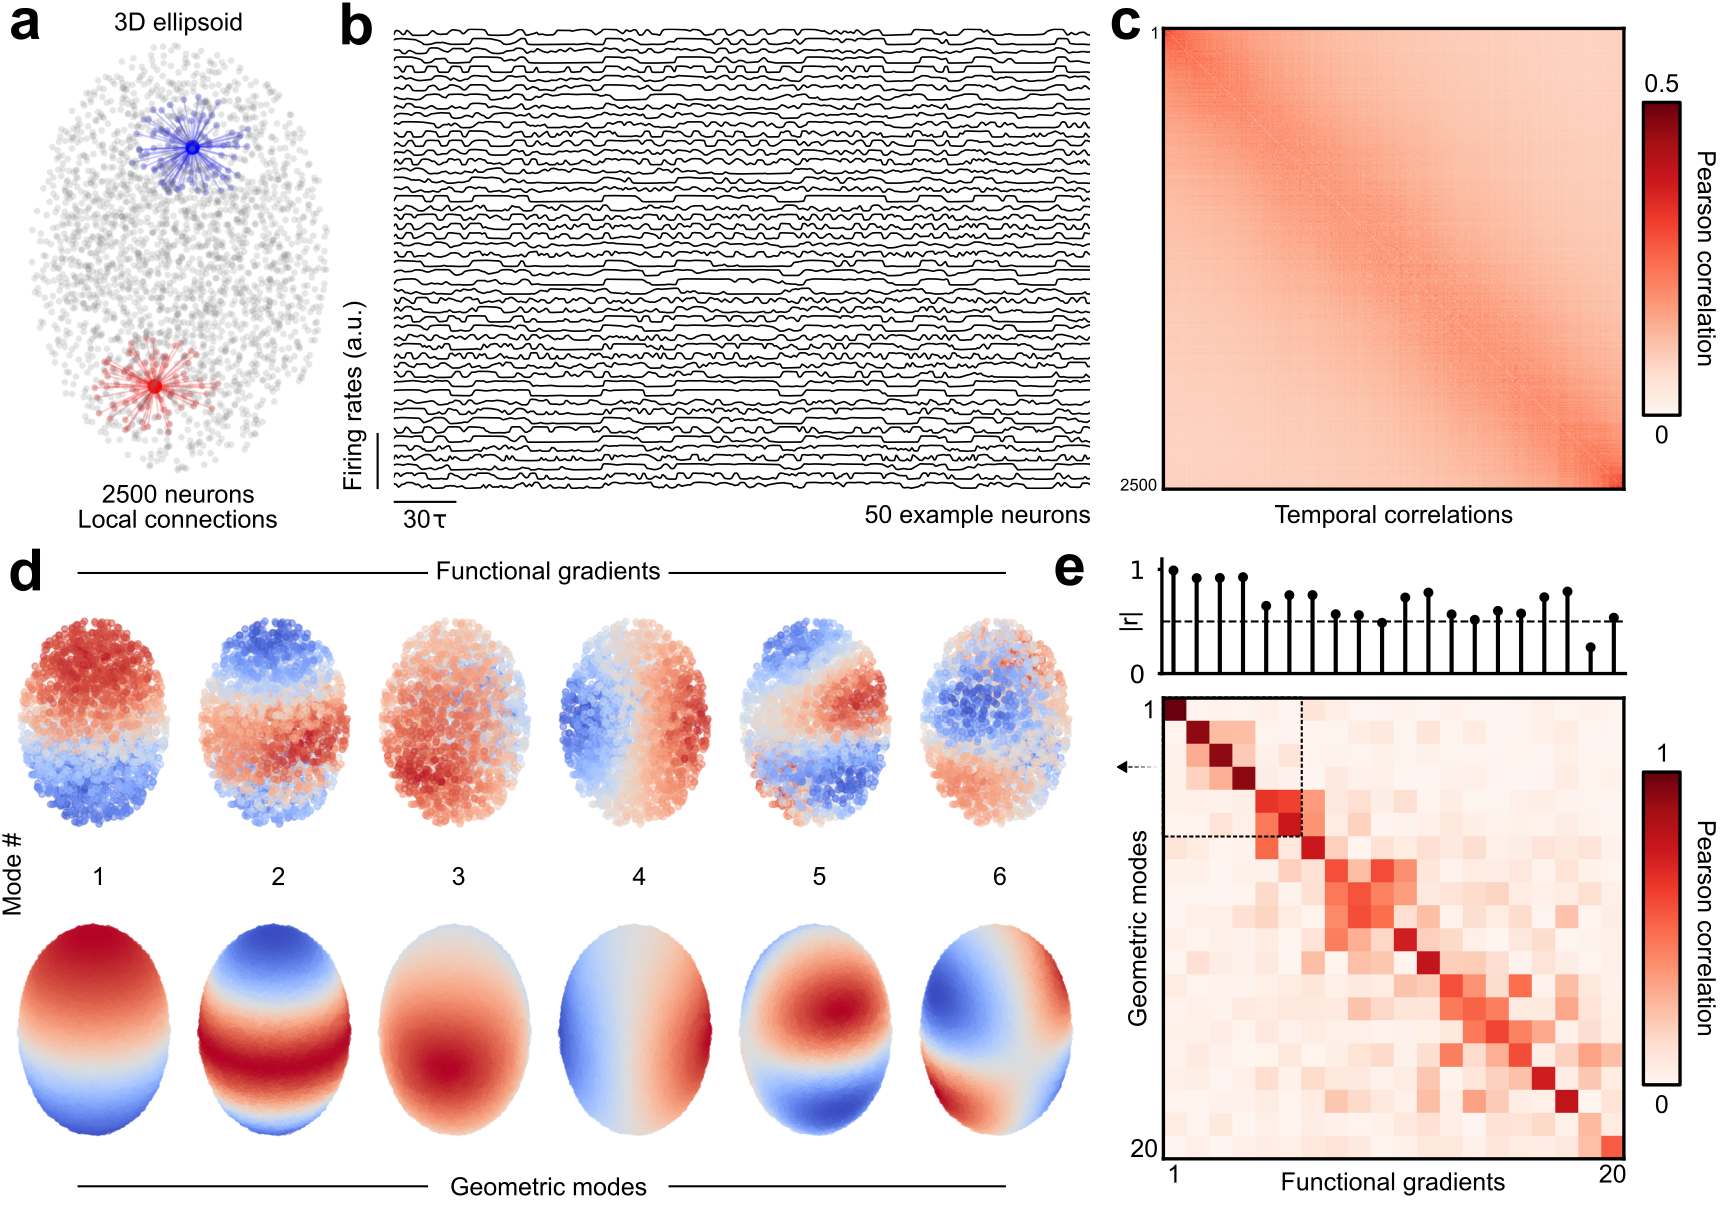
\includegraphics[width=0.95\textwidth]{Figures/figure1.png}
%    \caption{}
%    \label{fig1}
%\end{figure*}

\subsection*{Extending to arbitrary volumes}

\subsection*{Connection lengths constrain mode wavelengths}

\subsection*{Geometric gradients in other dynamical dynamical systems}

Spiking network

3D ising model?

Epidemic spreading?




\section*{Discussion}


\section*{Methods}


\newpage

\bibliographystyle{plain}
\bibliography{reference.bib}

\section*{Acknowledgements}

We acknowledge Calcul Québec and Digital Research Alliance of Canada for their technical support and computing infrastructures.

\section*{Author contributions}

\section*{Competing interests}

The authors declare no competing interests.

\end{multicols}

\newpage

\section*{Supplementary Material}


\end{document}